\pagestyle{plain}
\chapter{Blaise Pascal}
\label{chap:blaisePascal}

% \begin{figure}[t]
%  \centering
%  \includegraphics{./images/blaisePascal50pc.eps}
%  % Blaise_pascal.eps: 0x0 pixel, 300dpi, 0.00x0.00 cm, bb=-0 -0 299 313
%  \label{fig:Blaise Pascal}
% \end{figure}

\begin{flushright}
\textit{``El corazón tiene razones que la razón ignora.''}
\end{flushright}


{

\yinipar{B}laise Pascal\index{Blaise Pascal}, nacido el 19 de Junio de 1623 en Clemont y fallecido el 19 de Agosto de 1662 en París, es un importantísimo pensador: matemático físico, filósofo y escritor. Podemos afirmar que es ``un hombre e su época...''.
Pascal fue un importante racionalista a la vez que, según el paso de los años dedico enormes esfuerzos en ``racionalizar'' el Cristianismo y la figura e Dios. Es considerado un importante teólogo.

}

Trabajó en el campo de las matemáticas y diseño una máquina de cálculo ``Pascalina\index{Pascalina}'' capaz de realizar adiciones, con el tiempo, la propia máquina incorporó la operación de substracción.


Entre su más destacables estudios se encuentra la demostración del vació. \textit{Traité sur le vide} (Tratado sobre el vacío).


\paragraph*{Bibliografía:}
\begin{enumerate}[i.]
\item \textit{Essai pour les coniques} (1639) 
\item \textit{Experiences nouvelles touchant le vide} (1647)
\item \textit{Traité du triangle arithmétique} (1653)
\item \textit{Lettres provinciales} (1656–57)
\item \textit{De l'Esprit géométrique} (1657 o 1658)
\item \textit{Écrit sur la signature du formulaire} (1661)
\item \textit{Pensées} (Sin terminar)
\end{enumerate}


